\PassOptionsToPackage{unicode=true}{hyperref} % options for packages loaded elsewhere
\PassOptionsToPackage{hyphens}{url}
%
\documentclass[]{article}
\usepackage{lmodern}
\usepackage{amssymb,amsmath}
\usepackage{ifxetex,ifluatex}
\usepackage{fixltx2e} % provides \textsubscript
\ifnum 0\ifxetex 1\fi\ifluatex 1\fi=0 % if pdftex
  \usepackage[T1]{fontenc}
  \usepackage[utf8]{inputenc}
  \usepackage{textcomp} % provides euro and other symbols
\else % if luatex or xelatex
  \usepackage{unicode-math}
  \defaultfontfeatures{Ligatures=TeX,Scale=MatchLowercase}
\fi
% use upquote if available, for straight quotes in verbatim environments
\IfFileExists{upquote.sty}{\usepackage{upquote}}{}
% use microtype if available
\IfFileExists{microtype.sty}{%
\usepackage[]{microtype}
\UseMicrotypeSet[protrusion]{basicmath} % disable protrusion for tt fonts
}{}
\IfFileExists{parskip.sty}{%
\usepackage{parskip}
}{% else
\setlength{\parindent}{0pt}
\setlength{\parskip}{6pt plus 2pt minus 1pt}
}
\usepackage{hyperref}
\hypersetup{
            pdftitle={Practical 4: Visualisation using qplot()},
            pdfauthor={Laura Rodriguez Navas},
            pdfborder={0 0 0},
            breaklinks=true}
\urlstyle{same}  % don't use monospace font for urls
\usepackage[margin=1in]{geometry}
\usepackage{color}
\usepackage{fancyvrb}
\newcommand{\VerbBar}{|}
\newcommand{\VERB}{\Verb[commandchars=\\\{\}]}
\DefineVerbatimEnvironment{Highlighting}{Verbatim}{commandchars=\\\{\}}
% Add ',fontsize=\small' for more characters per line
\usepackage{framed}
\definecolor{shadecolor}{RGB}{248,248,248}
\newenvironment{Shaded}{\begin{snugshade}}{\end{snugshade}}
\newcommand{\AlertTok}[1]{\textcolor[rgb]{0.94,0.16,0.16}{#1}}
\newcommand{\AnnotationTok}[1]{\textcolor[rgb]{0.56,0.35,0.01}{\textbf{\textit{#1}}}}
\newcommand{\AttributeTok}[1]{\textcolor[rgb]{0.77,0.63,0.00}{#1}}
\newcommand{\BaseNTok}[1]{\textcolor[rgb]{0.00,0.00,0.81}{#1}}
\newcommand{\BuiltInTok}[1]{#1}
\newcommand{\CharTok}[1]{\textcolor[rgb]{0.31,0.60,0.02}{#1}}
\newcommand{\CommentTok}[1]{\textcolor[rgb]{0.56,0.35,0.01}{\textit{#1}}}
\newcommand{\CommentVarTok}[1]{\textcolor[rgb]{0.56,0.35,0.01}{\textbf{\textit{#1}}}}
\newcommand{\ConstantTok}[1]{\textcolor[rgb]{0.00,0.00,0.00}{#1}}
\newcommand{\ControlFlowTok}[1]{\textcolor[rgb]{0.13,0.29,0.53}{\textbf{#1}}}
\newcommand{\DataTypeTok}[1]{\textcolor[rgb]{0.13,0.29,0.53}{#1}}
\newcommand{\DecValTok}[1]{\textcolor[rgb]{0.00,0.00,0.81}{#1}}
\newcommand{\DocumentationTok}[1]{\textcolor[rgb]{0.56,0.35,0.01}{\textbf{\textit{#1}}}}
\newcommand{\ErrorTok}[1]{\textcolor[rgb]{0.64,0.00,0.00}{\textbf{#1}}}
\newcommand{\ExtensionTok}[1]{#1}
\newcommand{\FloatTok}[1]{\textcolor[rgb]{0.00,0.00,0.81}{#1}}
\newcommand{\FunctionTok}[1]{\textcolor[rgb]{0.00,0.00,0.00}{#1}}
\newcommand{\ImportTok}[1]{#1}
\newcommand{\InformationTok}[1]{\textcolor[rgb]{0.56,0.35,0.01}{\textbf{\textit{#1}}}}
\newcommand{\KeywordTok}[1]{\textcolor[rgb]{0.13,0.29,0.53}{\textbf{#1}}}
\newcommand{\NormalTok}[1]{#1}
\newcommand{\OperatorTok}[1]{\textcolor[rgb]{0.81,0.36,0.00}{\textbf{#1}}}
\newcommand{\OtherTok}[1]{\textcolor[rgb]{0.56,0.35,0.01}{#1}}
\newcommand{\PreprocessorTok}[1]{\textcolor[rgb]{0.56,0.35,0.01}{\textit{#1}}}
\newcommand{\RegionMarkerTok}[1]{#1}
\newcommand{\SpecialCharTok}[1]{\textcolor[rgb]{0.00,0.00,0.00}{#1}}
\newcommand{\SpecialStringTok}[1]{\textcolor[rgb]{0.31,0.60,0.02}{#1}}
\newcommand{\StringTok}[1]{\textcolor[rgb]{0.31,0.60,0.02}{#1}}
\newcommand{\VariableTok}[1]{\textcolor[rgb]{0.00,0.00,0.00}{#1}}
\newcommand{\VerbatimStringTok}[1]{\textcolor[rgb]{0.31,0.60,0.02}{#1}}
\newcommand{\WarningTok}[1]{\textcolor[rgb]{0.56,0.35,0.01}{\textbf{\textit{#1}}}}
\usepackage{graphicx,grffile}
\makeatletter
\def\maxwidth{\ifdim\Gin@nat@width>\linewidth\linewidth\else\Gin@nat@width\fi}
\def\maxheight{\ifdim\Gin@nat@height>\textheight\textheight\else\Gin@nat@height\fi}
\makeatother
% Scale images if necessary, so that they will not overflow the page
% margins by default, and it is still possible to overwrite the defaults
% using explicit options in \includegraphics[width, height, ...]{}
\setkeys{Gin}{width=\maxwidth,height=\maxheight,keepaspectratio}
\setlength{\emergencystretch}{3em}  % prevent overfull lines
\providecommand{\tightlist}{%
  \setlength{\itemsep}{0pt}\setlength{\parskip}{0pt}}
\setcounter{secnumdepth}{0}
% Redefines (sub)paragraphs to behave more like sections
\ifx\paragraph\undefined\else
\let\oldparagraph\paragraph
\renewcommand{\paragraph}[1]{\oldparagraph{#1}\mbox{}}
\fi
\ifx\subparagraph\undefined\else
\let\oldsubparagraph\subparagraph
\renewcommand{\subparagraph}[1]{\oldsubparagraph{#1}\mbox{}}
\fi

% set default figure placement to htbp
\makeatletter
\def\fps@figure{htbp}
\makeatother


\title{Practical 4: Visualisation using qplot()}
\author{Laura Rodriguez Navas}
\date{February 2020}

\begin{document}
\maketitle

Keratoconus is a disorder that affects the cornea through an abnormal
growth of collagen fibres. This makes the cornea become conical with an
important vision loss. There are many possible treatments, but one
common solution is the insertion of intrastromal corneal ring segments,
such that the cornea is flattened.

\hypertarget{todo-insert-img-in-latex}{%
\subsection{TODO insert img in LaTeX}\label{todo-insert-img-in-latex}}

\hypertarget{dataset}{%
\subsection{Dataset}\label{dataset}}

The file ``queratocono.csv'' includes information about 394 patients
with Keratoconus who were treated with ring placement. The variables
that were recorded are:

\begin{enumerate}
\def\labelenumi{\arabic{enumi}.}
\tightlist
\item
  K1: keratometry or main corneal curvature.
\item
  K2: perpendicular curvature to K1.
\item
  Ch: corneal hysteresis.
\item
  Na: number of rings (1 or 2).
\item
  Incision: angle in which the cornea is cut.
\item
  Prof: depth of the incision.
\item
  Diam: diameter of the incision.
\item
  Grosor: Incision thickness.
\item
  Longitud1: Angle of placement of the first ring (surgical parameter).
\item
  Longitud2: Angle of placement of the second ring (surgical parameter).
\item
  grosor1: Thickness of the first ring.
\item
  grosor2: Thickness of the second ring.
\item
  long1: arc length of the first ring.
\item
  long2: arc length of the second ring.
\item
  K1.salida: keratometry or main corneal curvature after the placement
  of the ring(s).
\item
  Astig: astigmatism curvature after the placement of the ring(s)
  (K1.salida -- K2.salida).
\end{enumerate}

A continuation, is provided a sample of the content of each variable of
dataset. It is also checked that there are no NA values and the dataset
is ordered by the column na.

\begin{Shaded}
\begin{Highlighting}[]
\KeywordTok{str}\NormalTok{(queratocono)}
\end{Highlighting}
\end{Shaded}

\begin{verbatim}
## 'data.frame':    394 obs. of  16 variables:
##  $ K1       : num  38.1 39.4 43.3 45.7 44.6 44.2 44.2 53.1 45.1 40.7 ...
##  $ K2       : num  48.6 53.6 50.4 50.1 50.4 44.8 45.8 53.8 52.5 44.5 ...
##  $ ch       : num  6.9 5.7 8.8 11.1 11.1 8.9 11.1 7.5 7.7 9.4 ...
##  $ na       : int  2 2 2 1 2 1 1 1 2 1 ...
##  $ Incision : int  60 140 120 30 60 180 130 60 60 30 ...
##  $ Prof     : int  390 400 381 370 440 327 380 400 380 477 ...
##  $ diam     : int  5 5 5 5 5 6 6 5 6 5 ...
##  $ grosor   : int  300 300 200 250 200 200 200 200 225 200 ...
##  $ Longitud1: int  90 105 120 160 120 150 210 160 120 160 ...
##  $ Longitud2: int  180 210 240 160 240 150 210 160 240 160 ...
##  $ grosor1  : int  300 300 200 250 200 200 200 200 200 200 ...
##  $ grosor2  : int  300 300 200 0 200 0 0 0 250 0 ...
##  $ long1    : int  90 90 120 160 120 150 210 160 90 160 ...
##  $ long2    : int  90 120 120 0 120 0 0 0 150 0 ...
##  $ K1.salida: num  35.5 42 42.7 45.8 44.4 42.8 43.1 48.7 45.7 39.8 ...
##  $ Astig    : num  10.1 8.9 3 1.9 2.9 2.3 3.9 2.8 3.2 3.8 ...
\end{verbatim}

\begin{Shaded}
\begin{Highlighting}[]
\KeywordTok{any}\NormalTok{(}\KeywordTok{is.na}\NormalTok{(queratocono))}
\end{Highlighting}
\end{Shaded}

\begin{verbatim}
## [1] FALSE
\end{verbatim}

\begin{Shaded}
\begin{Highlighting}[]
\NormalTok{queratocono <-}\StringTok{ }\NormalTok{queratocono[}\KeywordTok{order}\NormalTok{(queratocono}\OperatorTok{$}\NormalTok{na), ]}
\KeywordTok{str}\NormalTok{(queratocono)}
\end{Highlighting}
\end{Shaded}

\begin{verbatim}
## 'data.frame':    394 obs. of  16 variables:
##  $ K1       : num  45.7 44.2 44.2 53.1 40.7 35.4 51.5 40.6 49.5 44.9 ...
##  $ K2       : num  50.1 44.8 45.8 53.8 44.5 42 55.4 45.4 53.7 47.5 ...
##  $ ch       : num  11.1 8.9 11.1 7.5 9.4 8.2 10.1 8.6 7.2 7.6 ...
##  $ na       : int  1 1 1 1 1 1 1 1 1 1 ...
##  $ Incision : int  30 180 130 60 30 170 165 30 180 60 ...
##  $ Prof     : int  370 327 380 400 477 420 400 400 434 367 ...
##  $ diam     : int  5 6 6 5 5 5 6 6 5 5 ...
##  $ grosor   : int  250 200 200 200 200 250 200 250 200 200 ...
##  $ Longitud1: int  160 150 210 160 160 160 150 150 210 160 ...
##  $ Longitud2: int  160 150 210 160 160 160 150 150 210 160 ...
##  $ grosor1  : int  250 200 200 200 200 250 200 250 200 200 ...
##  $ grosor2  : int  0 0 0 0 0 0 0 0 0 0 ...
##  $ long1    : int  160 150 210 160 160 160 150 150 210 160 ...
##  $ long2    : int  0 0 0 0 0 0 0 0 0 0 ...
##  $ K1.salida: num  45.8 42.8 43.1 48.7 39.8 35.6 48.7 42.7 47.4 43.7 ...
##  $ Astig    : num  1.9 2.3 3.9 2.8 3.8 4 5.3 1.2 0.3 1.8 ...
\end{verbatim}

\hypertarget{analysis}{%
\subsection{Analysis}\label{analysis}}

In order to analyse the information in a visual way:

\begin{enumerate}
\def\labelenumi{\arabic{enumi}.}
\tightlist
\item
  Study the relation between K1 and K2 with smoother (by default and
  using linear regression).
\end{enumerate}

\begin{Shaded}
\begin{Highlighting}[]
\KeywordTok{qplot}\NormalTok{(K1, K2, }\DataTypeTok{data =}\NormalTok{ queratocono) }\OperatorTok{+}
\StringTok{  }\KeywordTok{geom_point}\NormalTok{() }\OperatorTok{+}\StringTok{ }
\StringTok{  }\KeywordTok{geom_smooth}\NormalTok{(}\DataTypeTok{method =} \StringTok{"loess"}\NormalTok{) }\OperatorTok{+}
\StringTok{  }\KeywordTok{xlab}\NormalTok{(}\StringTok{"K1"}\NormalTok{) }\OperatorTok{+}\StringTok{ }\KeywordTok{ylab}\NormalTok{(}\StringTok{"K2"}\NormalTok{)}
\end{Highlighting}
\end{Shaded}

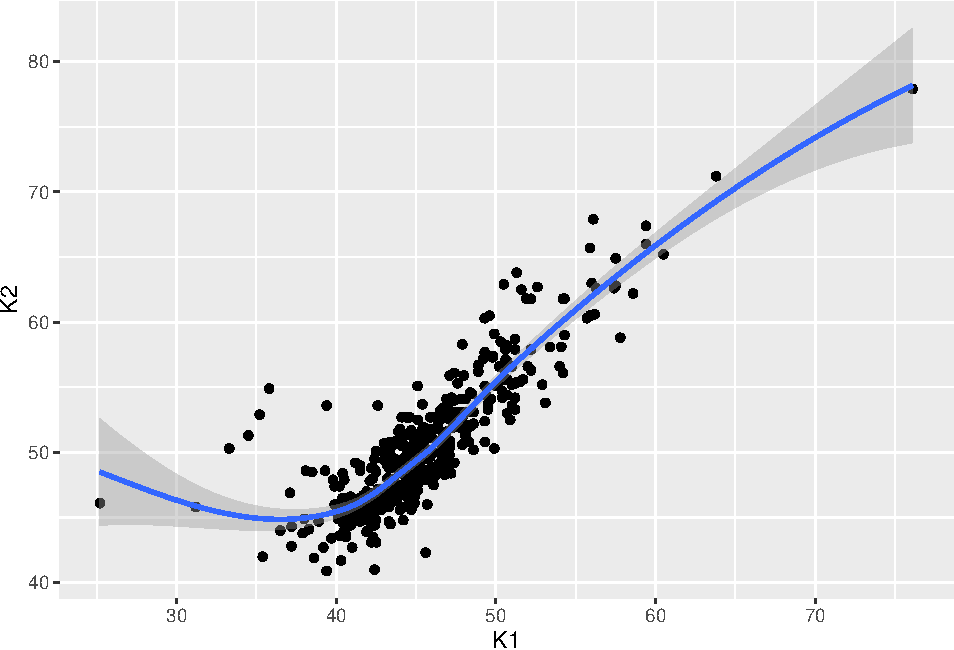
\includegraphics{document_files/figure-latex/unnamed-chunk-2-1.pdf}

\begin{Shaded}
\begin{Highlighting}[]
\KeywordTok{qplot}\NormalTok{(K1, K2, }\DataTypeTok{data =}\NormalTok{ queratocono) }\OperatorTok{+}
\StringTok{  }\KeywordTok{geom_point}\NormalTok{() }\OperatorTok{+}
\StringTok{  }\KeywordTok{geom_smooth}\NormalTok{(}\DataTypeTok{method =}\NormalTok{ lm) }\OperatorTok{+}
\StringTok{  }\KeywordTok{xlab}\NormalTok{(}\StringTok{"K1"}\NormalTok{) }\OperatorTok{+}\StringTok{ }\KeywordTok{ylab}\NormalTok{(}\StringTok{"K2"}\NormalTok{)}
\end{Highlighting}
\end{Shaded}

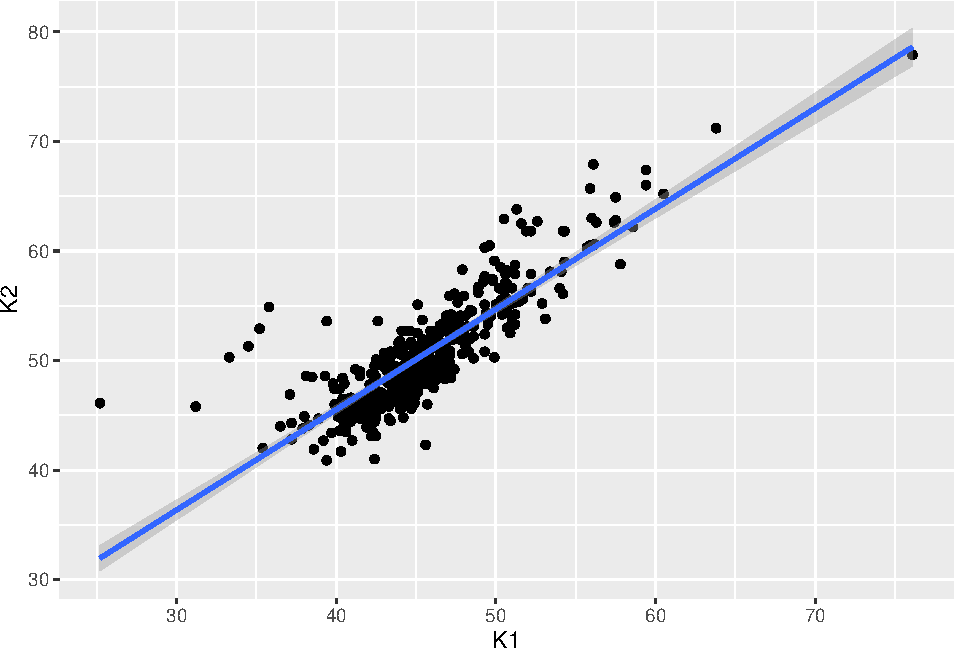
\includegraphics{document_files/figure-latex/unnamed-chunk-2-2.pdf}

\begin{enumerate}
\def\labelenumi{\arabic{enumi}.}
\setcounter{enumi}{1}
\tightlist
\item
  Study the relation between K1 and K2 distinguishing by factor na.
\end{enumerate}

\begin{Shaded}
\begin{Highlighting}[]
\KeywordTok{qplot}\NormalTok{(K1, K2, }\DataTypeTok{data =}\NormalTok{ queratocono, }\DataTypeTok{colour =} \KeywordTok{factor}\NormalTok{(na)) }\OperatorTok{+}
\StringTok{  }\KeywordTok{geom_point}\NormalTok{() }\OperatorTok{+}
\StringTok{  }\KeywordTok{geom_smooth}\NormalTok{(}\DataTypeTok{method =}\NormalTok{ lm) }\OperatorTok{+}
\StringTok{  }\KeywordTok{xlab}\NormalTok{(}\StringTok{"K1"}\NormalTok{) }\OperatorTok{+}\StringTok{ }\KeywordTok{ylab}\NormalTok{(}\StringTok{"K2"}\NormalTok{) }\OperatorTok{+}
\StringTok{  }\KeywordTok{ggtitle}\NormalTok{(}\StringTok{"Relation between K1 and K2"}\NormalTok{) }\OperatorTok{+}
\StringTok{  }\KeywordTok{theme_bw}\NormalTok{() }\OperatorTok{+}
\StringTok{  }\KeywordTok{theme}\NormalTok{(}\DataTypeTok{plot.title =} \KeywordTok{element_text}\NormalTok{(}\DataTypeTok{hjust =} \FloatTok{0.5}\NormalTok{))}
\end{Highlighting}
\end{Shaded}

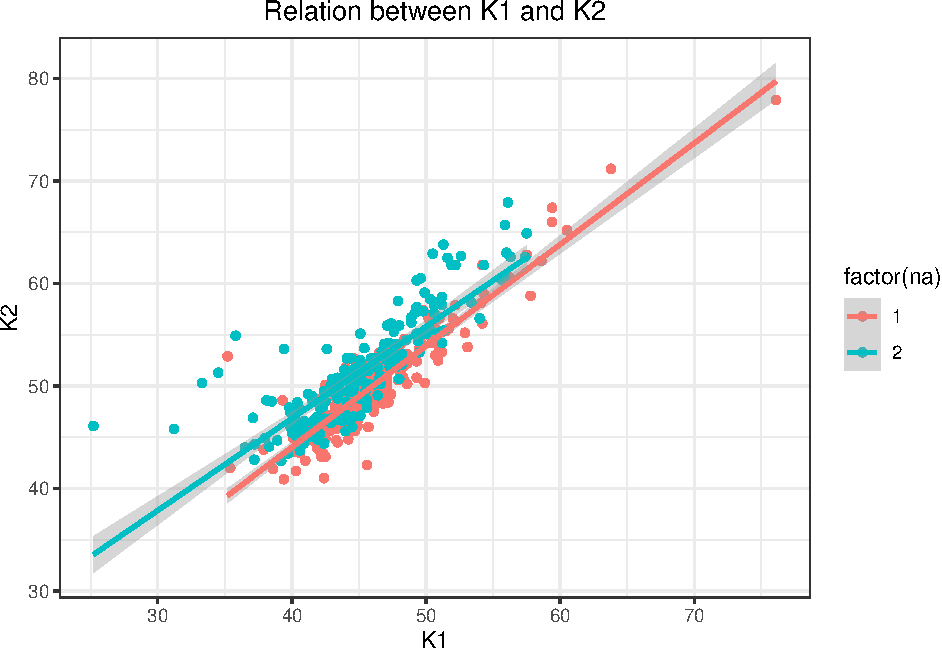
\includegraphics{document_files/figure-latex/unnamed-chunk-3-1.pdf}

\begin{enumerate}
\def\labelenumi{\arabic{enumi}.}
\setcounter{enumi}{2}
\tightlist
\item
  Study the relation between K1 and K1.salida.
\end{enumerate}

\begin{Shaded}
\begin{Highlighting}[]
\KeywordTok{qplot}\NormalTok{(K1, K1.salida, }\DataTypeTok{data =}\NormalTok{ queratocono) }\OperatorTok{+}
\StringTok{  }\KeywordTok{geom_point}\NormalTok{() }\OperatorTok{+}\StringTok{ }
\StringTok{  }\KeywordTok{xlab}\NormalTok{(}\StringTok{"K1"}\NormalTok{) }\OperatorTok{+}\StringTok{ }\KeywordTok{ylab}\NormalTok{(}\StringTok{"K1.salida"}\NormalTok{)}
\end{Highlighting}
\end{Shaded}

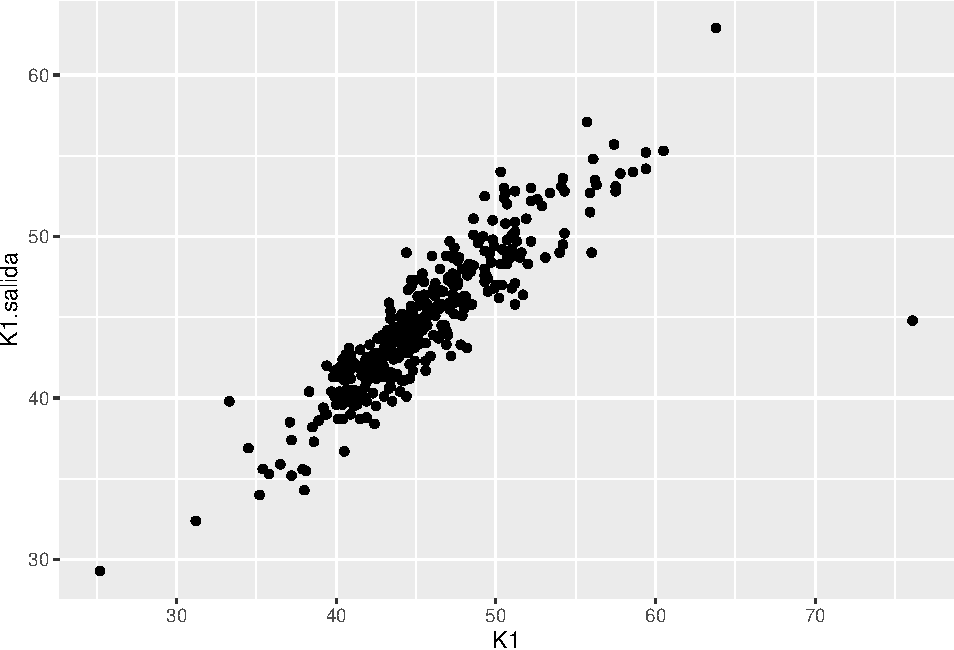
\includegraphics{document_files/figure-latex/unnamed-chunk-4-1.pdf}

\begin{enumerate}
\def\labelenumi{\arabic{enumi}.}
\setcounter{enumi}{3}
\tightlist
\item
  Build a histogram in terms of grosor (note that grosor should be taken
  as a factor) of the inserted ring.
\end{enumerate}

\begin{Shaded}
\begin{Highlighting}[]
\KeywordTok{ggplot}\NormalTok{(queratocono, }\KeywordTok{aes}\NormalTok{(}\KeywordTok{factor}\NormalTok{(grosor), }\DataTypeTok{geom =} \StringTok{"bar"}\NormalTok{ , }\DataTypeTok{fill =} \KeywordTok{factor}\NormalTok{(na))) }\OperatorTok{+}
\StringTok{  }\KeywordTok{geom_bar}\NormalTok{()}
\end{Highlighting}
\end{Shaded}

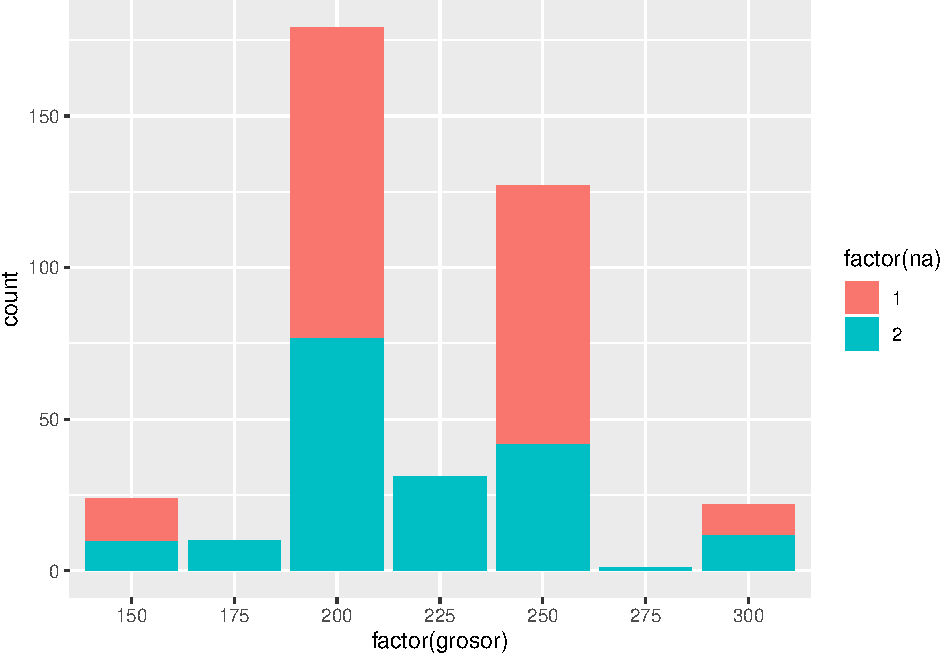
\includegraphics{document_files/figure-latex/unnamed-chunk-5-1.pdf}

\begin{enumerate}
\def\labelenumi{\arabic{enumi}.}
\setcounter{enumi}{4}
\tightlist
\item
  Build a scatter plot of the relation between K1 and K2 with
  ``faceting'' in terms of the parameters diam and na, by assigning
  different colours to the points according to the thickness (grosor) of
  the ring. In order to visualise all points correctly use a
  transparency of value 1/3.
\end{enumerate}

\begin{Shaded}
\begin{Highlighting}[]
\KeywordTok{qplot}\NormalTok{(K1, K2, }\DataTypeTok{data =}\NormalTok{ queratocono, }\DataTypeTok{colour =} \KeywordTok{factor}\NormalTok{(grosor), }\DataTypeTok{facets =}\NormalTok{ diam }\OperatorTok{~}\StringTok{ }\NormalTok{na, }
      \DataTypeTok{size =} \KeywordTok{I}\NormalTok{(}\DecValTok{1}\OperatorTok{/}\DecValTok{3}\NormalTok{)) }\OperatorTok{+}
\StringTok{      }\KeywordTok{geom_point}\NormalTok{() }\OperatorTok{+}\StringTok{ }
\StringTok{      }\KeywordTok{scale_shape_manual}\NormalTok{(}\DataTypeTok{values =} \DecValTok{0}\OperatorTok{:}\DecValTok{7}\NormalTok{) }\OperatorTok{+}
\StringTok{      }\KeywordTok{xlab}\NormalTok{(}\StringTok{"K1"}\NormalTok{) }\OperatorTok{+}\StringTok{ }\KeywordTok{ylab}\NormalTok{(}\StringTok{"K2"}\NormalTok{)}
\end{Highlighting}
\end{Shaded}

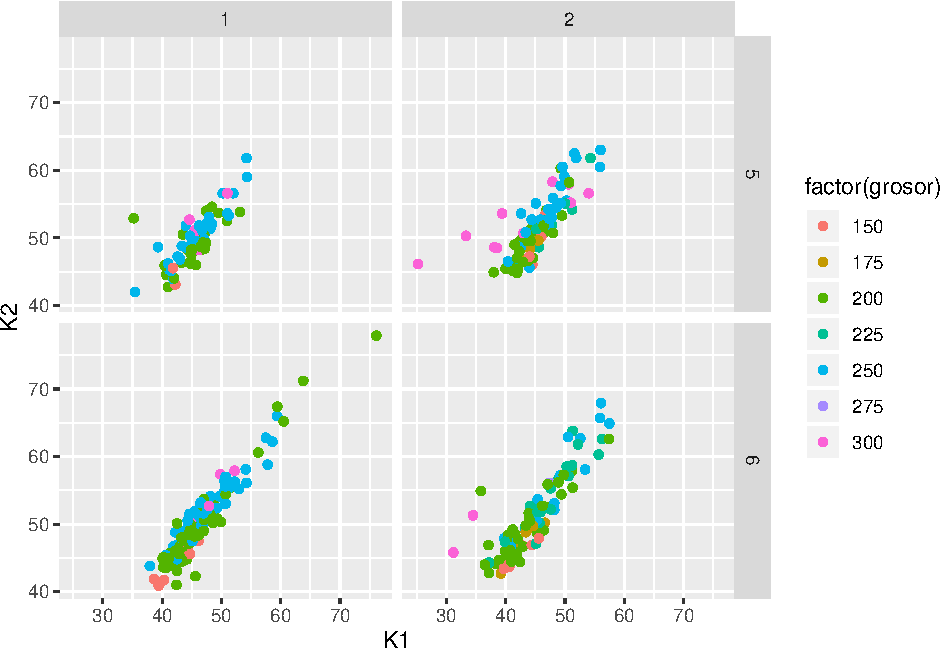
\includegraphics{document_files/figure-latex/unnamed-chunk-6-1.pdf}

\begin{enumerate}
\def\labelenumi{\arabic{enumi}.}
\setcounter{enumi}{5}
\tightlist
\item
  Create two boxplots that show a summary of the distributions of K1 and
  K2 (separately) with respect to the thickness (grosor).
\end{enumerate}

\begin{Shaded}
\begin{Highlighting}[]
\KeywordTok{qplot}\NormalTok{(}\KeywordTok{factor}\NormalTok{(grosor), K1, }\DataTypeTok{data =}\NormalTok{ queratocono, }\DataTypeTok{geom =} \StringTok{"boxplot"}\NormalTok{) }\OperatorTok{+}
\StringTok{  }\KeywordTok{xlab}\NormalTok{(}\StringTok{"factor(grosor)"}\NormalTok{) }\OperatorTok{+}\StringTok{ }\KeywordTok{ylab}\NormalTok{(}\StringTok{"K1"}\NormalTok{)}
\end{Highlighting}
\end{Shaded}

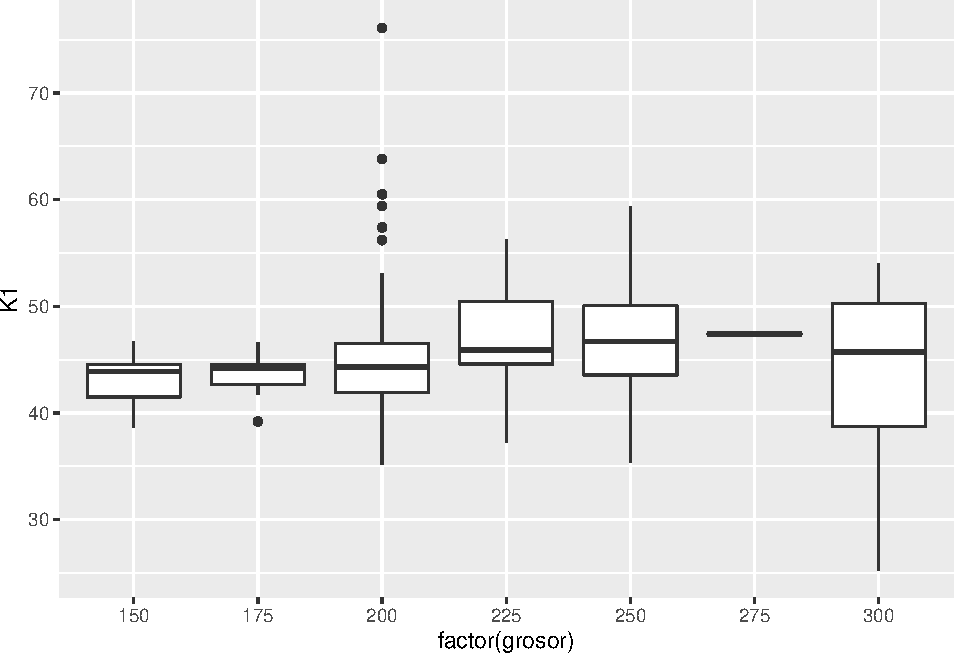
\includegraphics{document_files/figure-latex/unnamed-chunk-7-1.pdf}

\begin{Shaded}
\begin{Highlighting}[]
\KeywordTok{qplot}\NormalTok{(}\KeywordTok{factor}\NormalTok{(grosor), K2, }\DataTypeTok{data =}\NormalTok{ queratocono, }\DataTypeTok{geom =} \StringTok{"boxplot"}\NormalTok{) }\OperatorTok{+}
\StringTok{  }\KeywordTok{xlab}\NormalTok{(}\StringTok{"factor(grosor)"}\NormalTok{) }\OperatorTok{+}\StringTok{ }\KeywordTok{ylab}\NormalTok{(}\StringTok{"K2"}\NormalTok{)}
\end{Highlighting}
\end{Shaded}

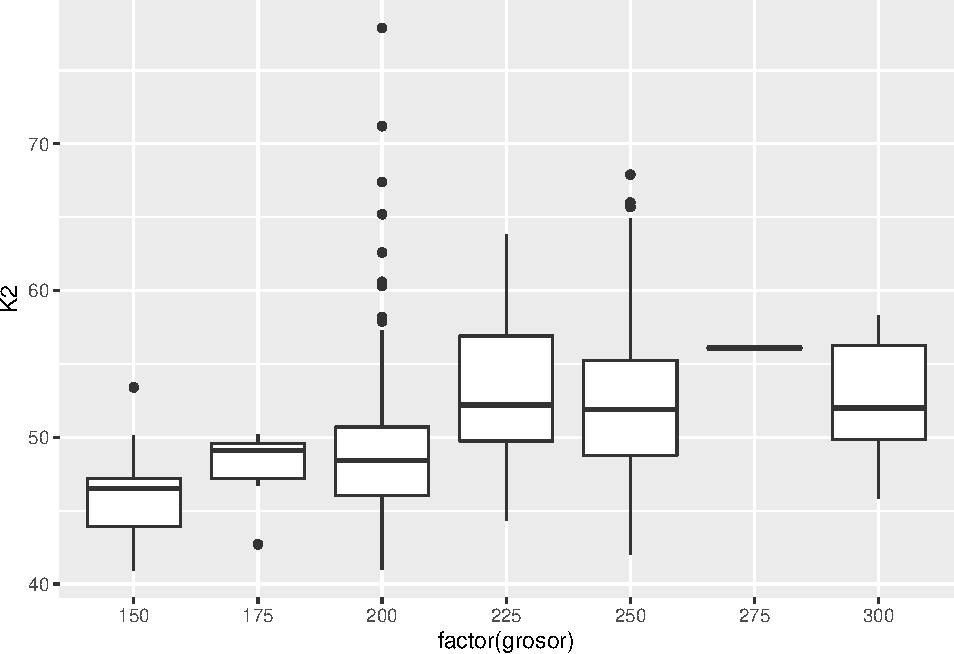
\includegraphics{document_files/figure-latex/unnamed-chunk-7-2.pdf}

\end{document}
